\providecommand{\main}{../..}
\documentclass[\main/main.tex]{subfiles}

%\graphicspath{ {\main/chapters/circuiti/}}

\begin{document}

\section{MOS Intro}

I MOS (Metal Oxide Semiconductor) sono dei tripoli a base di semiconduttori.

Sono ricavati da un substrato di semicoduttore drogato di un tipo in cui si realizzano due piazzole drogate in modo opposto e tra di esse vi si crea uno strato di ossido che funge da dielettrico.
Sopra alle piazzole ed al ossido si relizzano dei contatti metallici per poter collegare il MOS ai vari circuiti.

A seconda che si droghino le piazzole di tipo N o di tipo P si distinguono in NMOS e PMOS i quali sono sostanzialmente duali nel funzionamento.

I

\begin{figure}[H]
    \center
    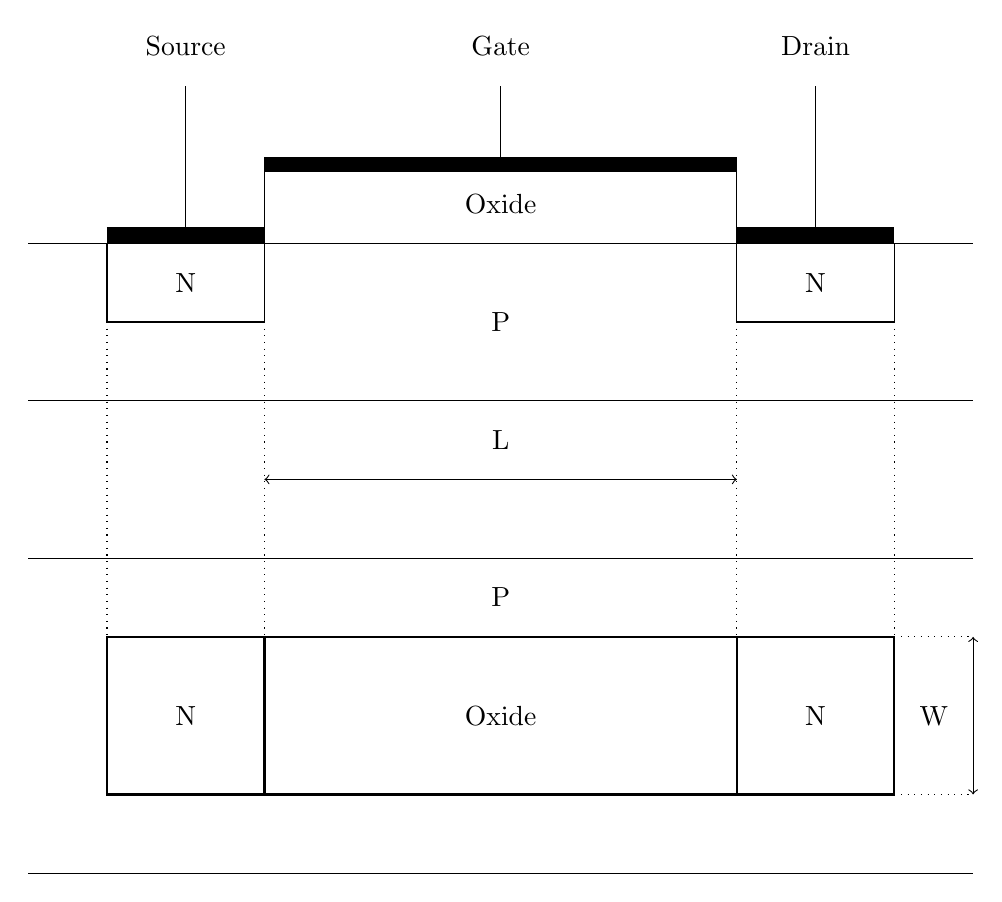
\begin{tikzpicture}
        % Silicon Top
        \draw (0,0)  -- (12,0);
        \draw (0,-2)  -- (12,-2);

        % Piazzola Source
        \draw (1,0)  -- (1,-1);
        \draw (1,-1) -- (3,-1);
        \draw (3,-1) -- (3,0);
        \draw [line width=0.2cm] (1,0.1)  -- (3,0.1);

        % Piazzola Drain
        \draw (9,0)  -- (9,-1);
        \draw (9,-1) -- (11,-1);
        \draw (11,-1) -- (11,0);
        \draw [line width=0.2cm] (9,0.1)  -- (11,0.1);

        % Gate
        \draw (3,0)  -- (3,1);
        \draw [line width=0.2cm] (3,1)  -- (9,1);
        \draw (9,1)  -- (9,0);

        % Gate Terminal
        \draw (6,1) -- (6,2);
        \node[] at (6,2.5) {Gate};

        % Source Terminal
        \draw (10,0) -- (10,2);
        \node[] at (10,2.5) {Drain};

        % Drain Terminal
        \draw (2,0) -- (2,2);
        \node[] at (2,2.5) {Source};

        % Letters
        \node[] at (2,-0.5) {N};
        \node[] at (10,-0.5) {N};
        \node[] at (6,-1) {P};
        \node[] at (6,0.5) {Oxide};

        %SEZIONE DAL ALTO

        % Silicon Top
        \draw (0,-4)  -- (12,-4);
        \draw (0,-8)  -- (12,-8);

        %Mos top
        \draw [fill=white, thick] (1,-5) rectangle (3,-7);
        \draw [fill=white, thick] (3,-5) rectangle (9,-7);
        \draw [fill=white, thick] (9,-5) rectangle (11,-7);

        % Letters
        \node[] at (2,-6) {N};
        \node[] at (10,-6) {N};
        \node[] at (6,-4.5) {P};
        \node[] at (6,-6) {Oxide};

        % L
        \draw [<->] (3,-3) -- (9,-3);
        \draw[dotted] (3,-1) -- (3,-5);
        \draw[dotted] (9,-1) -- (9,-5);
        \node[] at (6,-2.5) {L};

        % W
        \draw [<->] (12,-7) -- (12,-5);
        \draw[dotted] (11,-7) -- (12,-7);
        \draw[dotted] (11,-5) -- (12,-5);
        \node[] at (11.5,-6) {W};

        % projection dot
        \draw[dotted] (1,-1) -- (1,-5);
        \draw[dotted] (11,-1) -- (11,-5);

    \end{tikzpicture}
    \caption{Vista in sezione e dal alto di un NMOS}
\end{figure}


Definisco due caratteristiche del MOS:
\[K_n' = \frac{1}{2} \mu_n C_{ox}'\]
\[K_n = K_n' \left(\frac{W}{L}\right) = \frac{1}{2} \mu_n C_{ox}'\left(\frac{W}{L}\right)\]
\begin{align*}
    \mu_n   & \text{ e' la costante di mobilita' delle cariche libere}                      \\
    C_{ox}' & \text{ e' la capacita' del condesatore che si forma tra il gate ed il canale} \\
    W       & \text{ e' la larghezza del canale}                                            \\
    L       & \text{ e' la lunghezza del canale}
\end{align*}
\clearpage
\subsection{Regimi di Funzionamento di un MOS}
In realta' nelle zone di confine tra le piazzole ed il substrato si forma uno strato neutro poiche' a contatto da una parte con una zona drogata positivamente ed una drogata negativamente.

Quindi una immagine piu' reale del MOS e':

\begin{figure}[H]
    \center
    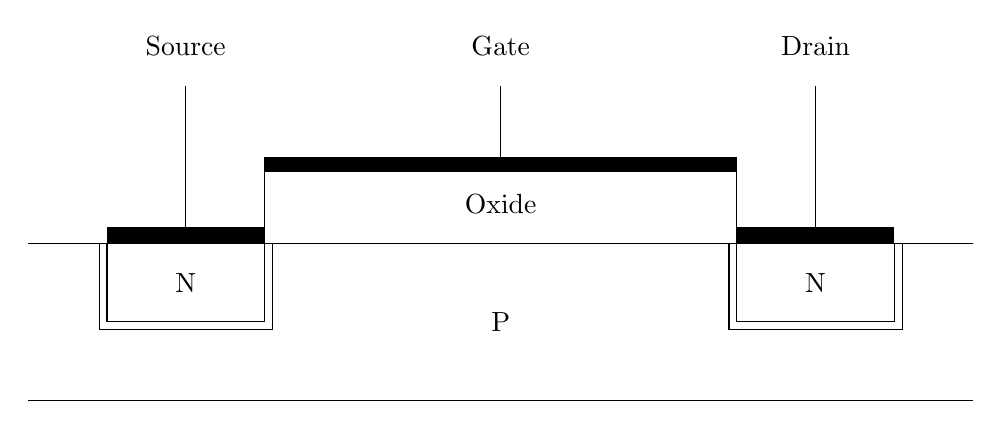
\begin{tikzpicture}
        % Silicon Top
        \draw (0,0)  -- (12,0);
        \draw (0,-2)  -- (12,-2);

        % Piazzola Source
        \draw (1,0)  -- (1,-1);
        \draw (1,-1) -- (3,-1);
        \draw (3,-1) -- (3,0);
        \draw [line width=0.2cm] (1,0.1)  -- (3,0.1);
        \draw (0.9,0)  -- (0.9,-1.1);
        \draw (0.9,-1.1) -- (3.1,-1.1);
        \draw (3.1,-1.1) -- (3.1,0);

        % Piazzola Drain
        \draw (9,0)  -- (9,-1);
        \draw (9,-1) -- (11,-1);
        \draw (11,-1) -- (11,0);
        \draw [line width=0.2cm] (9,0.1)  -- (11,0.1);
        \draw (8.9,0)  -- (8.9,-1.1);
        \draw (8.9,-1.1) -- (11.1,-1.1);
        \draw (11.1,-1.1) -- (11.1,0);

        % Gate
        \draw (3,0)  -- (3,1);
        \draw [line width=0.2cm] (3,1)  -- (9,1);
        \draw (9,1)  -- (9,0);

        % Gate Terminal
        \draw (6,1) -- (6,2);
        \node[] at (6,2.5) {Gate};

        % Source Terminal
        \draw (10,0) -- (10,2);
        \node[] at (10,2.5) {Drain};

        % Drain Terminal
        \draw (2,0) -- (2,2);
        \node[] at (2,2.5) {Source};

        % Letters
        \node[] at (2,-0.5) {N};
        \node[] at (10,-0.5) {N};
        \node[] at (6,-1) {P};
        \node[] at (6,0.5) {Oxide};

    \end{tikzpicture}
    \caption{Sezione di un NMOS con le zone neutre a vista}
\end{figure}

Normalmente nelle reallizzazzioni pratiche il substrato e' collegato al source

\begin{figure}[H]
    \center
    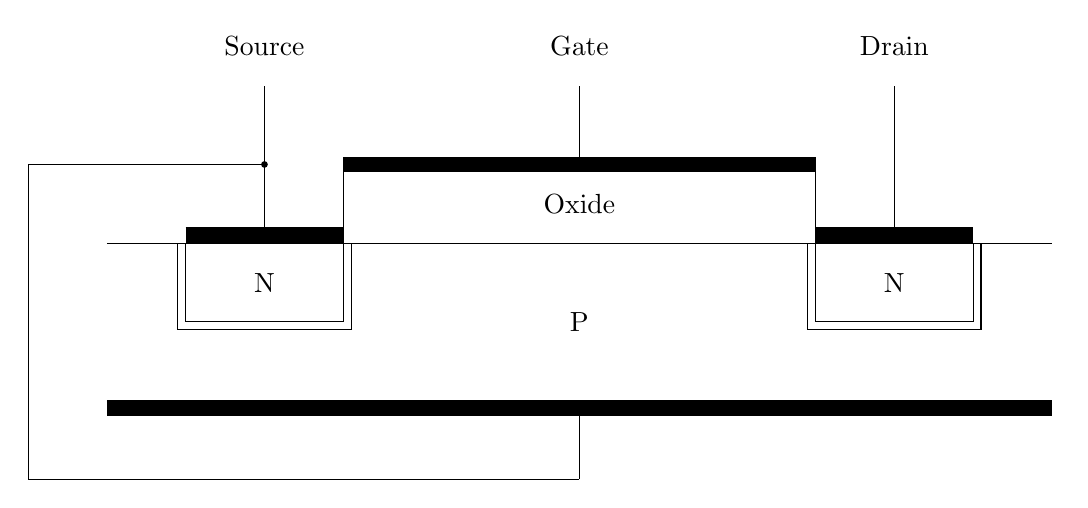
\begin{tikzpicture}
        % Silicon Top
        \draw (0,0)  -- (12,0);
        \draw (0,-2)  -- (12,-2);
        \draw [line width=0.2cm] (0,-2.1)  -- (12,-2.1);

        % Piazzola Source
        \draw (1,0)  -- (1,-1);
        \draw (1,-1) -- (3,-1);
        \draw (3,-1) -- (3,0);
        \draw [line width=0.2cm] (1,0.1)  -- (3,0.1);
        \draw (0.9,0)  -- (0.9,-1.1);
        \draw (0.9,-1.1) -- (3.1,-1.1);
        \draw (3.1,-1.1) -- (3.1,0);
        \draw (6,-2) -- (6,-3);
        \draw (6,-3) -- (-1,-3);
        \draw (-1,-3) -- (-1,1);
        \draw (-1,1) -- (2,1);

        \filldraw [black] (2,1) circle (1pt) node[below, black] {};


        % Piazzola Drain
        \draw (9,0)  -- (9,-1);
        \draw (9,-1) -- (11,-1);
        \draw (11,-1) -- (11,0);
        \draw [line width=0.2cm] (9,0.1)  -- (11,0.1);
        \draw (8.9,0)  -- (8.9,-1.1);
        \draw (8.9,-1.1) -- (11.1,-1.1);
        \draw (11.1,-1.1) -- (11.1,0);

        % Gate
        \draw (3,0)  -- (3,1);
        \draw [line width=0.2cm] (3,1)  -- (9,1);
        \draw (9,1)  -- (9,0);

        % Gate Terminal
        \draw (6,1) -- (6,2);
        \node[] at (6,2.5) {Gate};

        % Source Terminal
        \draw (10,0) -- (10,2);
        \node[] at (10,2.5) {Drain};

        % Drain Terminal
        \draw (2,0) -- (2,2);
        \node[] at (2,2.5) {Source};

        % Letters
        \node[] at (2,-0.5) {N};
        \node[] at (10,-0.5) {N};
        \node[] at (6,-1) {P};
        \node[] at (6,0.5) {Oxide};

    \end{tikzpicture}
    \caption{Sezione di un NMOS con source collegato al substrato}
\end{figure}


Ora se imponiamo a massa il Source ed il Drain ed iniziamo ad aumentare il potenziale ai capi del Gate si iniziano ad accumulare cariche sul Gate che come un condensatore attrae cariche opposte, sotto l'ossido, iniziando a formare una zona neutra.

Il MOS continua a rimaene spento e non vi puo' essere conduzione tra Source e Drain.

In realta' vi e' una piccola corrente di cross-conduzione ma tranquillamente approssimabile a 0 poiche' di diversi ordini di grandezza piu' piccola di quelle degli agltri regimi di funzionamento.

\[I_{DS} = 0\]

\begin{figure}[H]
    \center
    \begin{circuitikz}
        % Silicon Top
        \draw (0,0)  -- (12,0);
        \draw (0,-2)  -- (12,-2);
        \draw [line width=0.2cm] (0,-2.1)  -- (12,-2.1);

        % Piazzola Source
        \draw (1,0)  -- (1,-1);
        \draw (1,-1) -- (3,-1);
        \draw (3,-1) -- (3,0);
        \draw [line width=0.2cm] (1,0.1)  -- (3,0.1);
        \draw (0.9,0)  -- (0.9,-1.1);
        \draw (0.9,-1.1) -- (3.1,-1.1);
        \draw (3.1,-1.1) -- (3.1,-0.1);

        % Piazzola Drain
        \draw (9,0)  -- (9,-1);
        \draw (9,-1) -- (11,-1);
        \draw (11,-1) -- (11,0);
        \draw [line width=0.2cm] (9,0.1)  -- (11,0.1);
        \draw (8.9,-0.1)  -- (8.9,-1.1);
        \draw (8.9,-1.1) -- (11.1,-1.1);
        \draw (11.1,-1.1) -- (11.1,0);
        \draw (6,-2) -- (6,-3);
        \draw (6,-3) -- (-1,-3);
        \draw (-1,-3) -- (-1,1);
        \draw (-1,1) -- (2,1);

        \filldraw [black] (2,1) circle (1pt) node[below, black] {};

        % Gate
        \draw (3,0)  -- (3,1);
        \draw [line width=0.2cm] (3,1)  -- (9,1);
        \draw (9,1)  -- (9,0);
        \draw (3.1,-0.1)  -- (8.9,-0.1);

        % Gate Terminal
        \draw (6,1) -- (6,2);
        \node[] at (6,2.5) {Gate};

        % Source Terminal
        \draw (10,0) -- (10,3.5);
        \node[] at (11,2.5) {Drain};

        % Drain Terminal
        \draw (2,0) -- (2,3.5);
        \node[] at (1,2.5) {Source};

        % Letters
        \node[] at (2,-0.5) {N};
        \node[] at (10,-0.5) {N};
        \node[] at (6,-1) {P};
        \node[] at (6,0.5) {Oxide};

        \draw (6,2) to[american voltage source, v_<= $V_{GS}$] (2,2);

        \filldraw [black] (2,2) circle (1pt) node[below, black] {};

        \draw (2,3.5) -- (10,3.5);

    \end{circuitikz}
    \caption{Sezione di un NMOS al aumentare del potenziale sul Gate}
\end{figure}

Una volta che il Potenziale al Gate ha superato una Tensione di Soglia $V_t$ ( che e' una caratteritica del MOS) si inizia a formare un canale polarizzato come le piazzole il quale avendo cairche libere puo' essere attraversato da una corrente tra Source e Drain $I_{DS}$.

In questa situazione in cui vi e' il canale da entrambi i lati si dice che il MOS sta lavorando in regime Ohmmico.

\[I_{DS} = K_n \left[ 2 \left(V_{GS} - V_t \right)V_{DS} - V_{DS}^2 \right]\]

\begin{figure}[H]
    \center
    \begin{circuitikz}
        % Silicon Top
        \draw (0,0)  -- (12,0);
        \draw (0,-2)  -- (12,-2);
        \draw [line width=0.2cm] (0,-2.1)  -- (12,-2.1);

        % Piazzola Source
        \draw (1,0)  -- (1,-1);
        \draw (1,-1) -- (3,-1);
        \draw (3,-1) -- (3,-0.4);
        \draw [line width=0.2cm] (1,0.1)  -- (3,0.1);
        \draw (0.9,0)  -- (0.9,-1.1);
        \draw (0.9,-1.1) -- (3.1,-1.1);
        \draw (3.1,-1.1) -- (3.1,-0.5);

        % Piazzola Drain
        \draw (9,-0.4)  -- (9,-1);
        \draw (9,-1) -- (11,-1);
        \draw (11,-1) -- (11,0);
        \draw [line width=0.2cm] (9,0.1)  -- (11,0.1);
        \draw (8.9,-0.5)  -- (8.9,-1.1);
        \draw (8.9,-1.1) -- (11.1,-1.1);
        \draw (11.1,-1.1) -- (11.1,0);
        \draw (6,-2) -- (6,-3);
        \draw (6,-3) -- (-1,-3);
        \draw (-1,-3) -- (-1,1);
        \draw (-1,1) -- (2,1);

        \filldraw [black] (2,1) circle (1pt) node[below, black] {};

        % Gate
        \draw (3,0)  -- (3,1);
        \draw [line width=0.2cm] (3,1)  -- (9,1);
        \draw (9,1)  -- (9,0);
        \draw (3,-0.4)  -- (9,-0.4);
        \draw (3.1,-0.5)  -- (8.9,-0.5);

        % Gate Terminal
        \draw (6,1) -- (6,2);
        \node[] at (6,2.5) {Gate};

        % Source Terminal
        \draw (10,0) -- (10,3.5);
        \node[] at (11,2.5) {Drain};

        % Drain Terminal
        \draw (2,0) -- (2,3.5);
        \node[] at (1,2.5) {Source};

        % Letters
        \node[] at (2,-0.5) {N};
        \node[] at (10,-0.5) {N};
        \node[] at (6,-1) {P};
        \node[] at (6,0.5) {Oxide};

        \draw (6,2) to[american voltage source, v_<= $V_{GS}$] (2,2);

        \filldraw [black] (2,2) circle (1pt) node[below, black] {};

        \draw (2,3.5) -- (10,3.5);

        \draw[dotted] (3,0) -- (3,-0.5);
        \draw[dotted] (9,0) -- (9,-0.5);

    \end{circuitikz}
    \caption{Sezione di un NMOS al aumentare del potenziale sul Gate}
\end{figure}

Ora se impongo una tensione $V_{DS}$ il canale inizia ad essere attratto verso il drain quindi il canale non e' piu' parallelo al' ossido ma diventa.


\begin{figure}[H]
    \center
    \begin{circuitikz}
        % Silicon Top
        \draw (0,0)  -- (12,0);
        \draw (0,-2)  -- (12,-2);
        \draw [line width=0.2cm] (0,-2.1)  -- (12,-2.1);

        % Piazzola Source
        \draw (1,0)  -- (1,-1);
        \draw (1,-1) -- (3,-1);
        \draw (3,-1) -- (3,-0.6);
        \draw [line width=0.2cm] (1,0.1)  -- (3,0.1);
        \draw (0.9,0)  -- (0.9,-1.1);
        \draw (0.9,-1.1) -- (3.1,-1.1);
        \draw (3.1,-1.1) -- (3.1,-0.7);

        % Piazzola Drain
        \draw (9,-0.2)  -- (9,-1);
        \draw (9,-1) -- (11,-1);
        \draw (11,-1) -- (11,0);
        \draw [line width=0.2cm] (9,0.1)  -- (11,0.1);
        \draw (8.9,-0.3)  -- (8.9,-1.1);
        \draw (8.9,-1.1) -- (11.1,-1.1);
        \draw (11.1,-1.1) -- (11.1,0);
        \draw (6,-2) -- (6,-3);
        \draw (6,-3) -- (-1,-3);
        \draw (-1,-3) -- (-1,1);
        \draw (-1,1) -- (2,1);

        \filldraw [black] (2,1) circle (1pt) node[below, black] {};

        % Gate
        \draw (3,0)  -- (3,1);
        \draw [line width=0.2cm] (3,1)  -- (9,1);
        \draw (9,1)  -- (9,0);
        \draw (3,-0.6)  -- (9,-0.2);
        \draw (3.1,-0.7)  -- (8.9,-0.3);

        % Gate Terminal
        \draw (6,1) -- (6,2);
        \node[] at (6,2.5) {Gate};

        % Source Terminal
        \draw (10,0) -- (10,3.5);
        \node[] at (11,2.5) {Drain};

        % Drain Terminal
        \draw (2,0) -- (2,3.5);
        \node[] at (1,2.5) {Source};

        % Letters
        \node[] at (2,-0.5) {N};
        \node[] at (10,-0.5) {N};
        \node[] at (6,-1) {P};
        \node[] at (6,0.5) {Oxide};

        \draw (6,2) to[american voltage source, v_<= $V_{GS}$] (2,2);

        \filldraw [black] (2,2) circle (1pt) node[below, black] {};

        \draw (10,3.5)  to[american voltage source, v_<= $V_{DS}$] (2,3.5);

        \draw[dotted] (3,0) -- (3,-0.6);
        \draw[dotted] (9,0) -- (9,-0.2);

    \end{circuitikz}
    \caption{Sezione di un NMOS applicando una tnesione tra Source e Drain}
\end{figure}

Se la tensione $V_{DS} > V_{GS} - V_t$ allora si verifica il fenomeno del pinch-off nel quale il canale e' totalmente spostato verso un lato ed a questo punto la resistivita' del canale non dipende piu' dalla $V_{DS}$ ma solo dalla $V_{GS}$.

\[ I_{DS} = K_n \left( V_{GS} - V_t \right)^2\]

Si dice che il MOS si trova in regime di saturazione.

\begin{figure}[H]
    \center
    \begin{circuitikz}
        % Silicon Top
        \draw (0,0)  -- (12,0);
        \draw (0,-2)  -- (12,-2);
        \draw [line width=0.2cm] (0,-2.1)  -- (12,-2.1);

        % Piazzola Source
        \draw (1,0)  -- (1,-1);
        \draw (1,-1) -- (3,-1);
        \draw (3,-1) -- (3,-1);
        \draw [line width=0.2cm] (1,0.1)  -- (3,0.1);
        \draw (0.9,0)  -- (0.9,-1.1);
        \draw (0.9,-1.1) -- (3.1,-1.1);
        \draw (3.1,-1.1) -- (3.1,-1.1);

        % Piazzola Drain
        \draw (9,-0)  -- (9,-1);
        \draw (9,-1) -- (11,-1);
        \draw (11,-1) -- (11,0);
        \draw [line width=0.2cm] (9,0.1)  -- (11,0.1);
        \draw (8.9,-0.1)  -- (8.9,-1.1);
        \draw (8.9,-1.1) -- (11.1,-1.1);
        \draw (11.1,-1.1) -- (11.1,0);
        \draw (6,-2) -- (6,-3);
        \draw (6,-3) -- (-1,-3);
        \draw (-1,-3) -- (-1,1);
        \draw (-1,1) -- (2,1);

        \filldraw [black] (2,1) circle (1pt) node[below, black] {};

        % Gate
        \draw (3,0)  -- (3,1);
        \draw [line width=0.2cm] (3,1)  -- (9,1);
        \draw (9,1)  -- (9,0);
        \draw (3,-1)  -- (9,-0);
        \draw (3.1,-1.1)  -- (8.9,-0.1);

        % Gate Terminal
        \draw (6,1) -- (6,2);
        \node[] at (6,2.5) {Gate};

        % Source Terminal
        \draw (10,0) -- (10,3.5);
        \node[] at (11,2.5) {Drain};

        % Drain Terminal
        \draw (2,0) -- (2,3.5);
        \node[] at (1,2.5) {Source};

        % Letters
        \node[] at (2,-0.5) {N};
        \node[] at (10,-0.5) {N};
        \node[] at (6,-1) {P};
        \node[] at (6,0.5) {Oxide};

        \draw (6,2) to[american voltage source, v_<= $V_{GS}$] (2,2);

        \filldraw [black] (2,2) circle (1pt) node[below, black] {};

        \draw (10,3.5)  to[american voltage source, v_<= $V_{DS}$] (2,3.5);


        \draw[dotted] (3,0) -- (3,-1);

        \draw [->] (8,-1) -- (8.8,-0.2);

        \node[] at (8,-1.3) {Pintchoff};

    \end{circuitikz}
    \caption{Sezione di un NMOS in saturazione}
\end{figure}

Quindi riassumendo Le caratteristiche del MOS sono:

\begin{figure}[H]
    \centering
    \begin{subfigure}{.5\textwidth}
        \centering
        \begin{tikzpicture}[axis/.style={very thick, ->, >=stealth'} ]
            \draw[axis] (0,0)  -- (6,0) node(xline)[right] {$V_{DS}$};
            \draw[axis] (0,0) -- (0,5) node(yline)[above] {$I_{DS}$};

            \draw[dotted] (2,0) -- (2,5);
            \draw[dotted] (0,4) -- (2,4);
            \filldraw [black] (2,0) circle (1pt) node[below, black] {$V_{GS} - V_t$};

            \filldraw [blue] (0,0) circle (1pt);

            \draw[scale=1,domain=0:2,smooth,variable=\x,blue] plot ({\x},{4*\x-\x^2});
            \draw[scale=1,domain=2:6,smooth,variable=\x,blue] plot ({\x},{4});

            \filldraw [black] (0, 4) circle (1pt) node[above right, black] {$I_{SAT}$};

            \node[] at (1,4.5) {Ohm};
            \node[] at (4,4.5) {Saturazione};

        \end{tikzpicture}
    \end{subfigure}
    \begin{subfigure}{.5\textwidth}
        \centering
        \begin{tikzpicture}[axis/.style={very thick, ->, >=stealth'} ]
            \draw[axis] (0,0)  -- (6,0) node(xline)[right] {$V_{GS}$};
            \draw[axis] (0,0) -- (0,5) node(yline)[above] {$I_{DS}$};

            \draw[dotted] (2,0) -- (2,5);

            \filldraw [black] (2,0) circle (1pt) node[below, black] {$V_t$};

            \draw[scale=1,domain=2:4,smooth,variable=\x,blue] plot ({\x},{\x-2)^2});

            \node[] at (1,5) {Spento};
            \node[] at (4,5) {Acceso};

        \end{tikzpicture}
    \end{subfigure}
\end{figure}

\clearpage
\section{NMOS ed PMOS}
Esistono due tipi duali e complementari di MOS: NMOS (Piu' usati e con caratteristiche migliori) e i PMOS.

\subsection{NMOS}

\begin{center}
    \begin{circuitikz}
        \draw(0,0) node[nmos] (mos) {}
        (mos.gate) node[anchor=east] {G}
        (mos.drain) node[anchor=south] {D}
        (mos.source) node[anchor=north] {S};
        \draw (mos.drain) to[open, v^<=$V_{DS}$] (mos.source);
        \draw (mos.gate)  to[open, v_<=$V_{GS}$] (mos.source);
        \draw (mos.gate)  to[open, v^<=$V_{GD}$] (mos.drain);
    \end{circuitikz}
\end{center}

\[K_n = K_n' \left(\frac{W}{L}\right) = \frac{1}{2} \mu_n C_{ox}'\left(\frac{W}{L}\right)\]

Il NMOS e' spento se la $V_{GS} < V_t$

e quindi la corrente
\[I_{DS} = 0\]


Il NMOS e' in regime ohmico o lineare se $V_{DS} < V_{GS} - V_t$

e quindi la corrente

\[I_{DS} = K_n \left[ 2 \left(V_{GS} - V_t \right)V_{DS} - V_{DS}^2 \right]\]


Il NMOS e' in zona di saturazione se $V_{DS} > V_{GS} - V_t$

e quindi la corrente

\[ I_{DS} = K_n \left( V_{GS} - V_t \right)^2\]

\begin{figure}[H]
    \centering
    \begin{subfigure}{.5\textwidth}
        \centering
        \begin{tikzpicture}[
                axis/.style={very thick, ->, >=stealth'} ]
            \draw[axis] (0,0)  -- (6,0) node(xline)[right] {$V_{DS}$};
            \draw[axis] (0,0) -- (0,5) node(yline)[above] {$I_{DS}$};

            \draw[dotted] (2,0) -- (2,5);
            \draw[dotted] (0,4) -- (2,4);
            \filldraw [black] (2,0) circle (1pt) node[below, black] {$V_{GS} - V_t$};

            \filldraw [blue] (0,0) circle (1pt);

            \draw[scale=1,domain=0:2,smooth,variable=\x,blue] plot ({\x},{(4*\x-\x^2});
            \draw[scale=1,domain=2:6,smooth,variable=\x,blue] plot ({\x},{4});

            \filldraw [black] (0, 4) circle (1pt) node[above right, black] {$I_{SAT}$};

            \node[] at (1,4.5) {Ohm};
            \node[] at (4,4.5) {Saturazione};

        \end{tikzpicture}
    \end{subfigure}%
    \begin{subfigure}{.5\textwidth}
        \centering
        \begin{tikzpicture}[
                axis/.style={very thick, ->, >=stealth'} ]
            \draw[axis] (0,0)  -- (6,0) node(xline)[right] {$V_{GS}$};
            \draw[axis] (0,0) -- (0,5) node(yline)[above] {$I_{DS}$};

            \draw[dotted] (2,0) -- (2,5);

            \filldraw [black] (2,0) circle (1pt) node[below, black] {$V_t$};

            \draw[scale=1,domain=2:4,smooth,variable=\x,blue] plot ({\x},{(\x-2)^2});

            \node[] at (1,5) {Spento};
            \node[] at (4,5) {Acceso};

        \end{tikzpicture}
    \end{subfigure}
\end{figure}

\clearpage
\subsection{PMOS}

\begin{center}
    \begin{circuitikz} \draw
        (0,0) node[pmos] (mos) {}
        (mos.gate) node[anchor=east] {G}
        (mos.drain) node[anchor=north] {D}
        (mos.source) node[anchor=south] {S};
        \draw (mos.drain) to[open, v_>=$V_{SD}$] (mos.source);
        \draw (mos.gate)  to[open, v^>=$V_{SG}$] (mos.source);
        \draw (mos.gate)  to[open, v_>=$V_{DG}$] (mos.drain);
    \end{circuitikz}
\end{center}

[ATTENZIONE AI SEGNI]
\[K_p = K_p' \left(\frac{W}{L}\right) = \frac{1}{2} \mu_p C_{ox}'\left(\frac{W}{L}\right)\]

Il PMOS e' spento se la $\left|V_{GS}\right| < \left|V_t\right|$

e quindi la corrente
\[I_{SD} = 0\]


Il PMOS e' in regime ohmico o lineare se $V_{SD} < V_{SG} - V_t$

e quindi la corrente

\[I_{SD} = K_p \left[ 2 \left(V_{SG} - V_t \right)V_{SD} - V_{SD}^2 \right]\]


Il PMOS e' in zona di saturazione se $V_{SD} > V_{SG} - V_t$

e quindi la corrente

\[ I_{SD} = K_p \left( V_{SG} - V_t \right)^2\]

\begin{figure}
    \begin{subfigure}{.5\textwidth}
        \centering
        \begin{tikzpicture}[axis/.style={very thick, ->, >=stealth'} ]
            \draw[axis] (0,0)  -- (6,0) node(xline)[right] {$V_{SD}$};
            \draw[axis] (0,0) -- (0,5) node(yline)[above] {$I_{SD}$};

            \draw[dotted] (2,0) -- (2,5);
            \draw[dotted] (0,4) -- (2,4);
            \filldraw [black] (2,0) circle (1pt) node[below, black] {$V_{SG} - V_t$};

            \filldraw [blue] (0,0) circle (1pt);

            \draw[scale=1,domain=0:2,smooth,variable=\x,blue] plot ({\x},{(4*\x-\x^2});
            \draw[scale=1,domain=2:6,smooth,variable=\x,blue] plot ({\x},{4});

            \filldraw [black] (0, 4) circle (1pt) node[above right, black] {$I_{SAT}$};

            \node[] at (1,4.5) {Ohm};
            \node[] at (4,4.5) {Saturazione};

        \end{tikzpicture}
    \end{subfigure}%
    \begin{subfigure}{.5\textwidth}
        \centering
        \begin{tikzpicture}[axis/.style={very thick, ->, >=stealth'} ]
            \draw[axis] (0,0)  -- (6,0) node(xline)[right] {$V_{SG}$};
            \draw[axis] (0,0) -- (0,5) node(yline)[above] {$I_{SD}$};

            \draw[dotted] (2,0) -- (2,5);

            \filldraw [black] (2,0) circle (1pt) node[below, black] {$V_t$};

            \draw[scale=1,domain=2:4,smooth,variable=\x,blue] plot ({\x},{(\x-2)^2});

            \node[] at (1,5) {Spento};
            \node[] at (4,5) {Acceso};

        \end{tikzpicture}
    \end{subfigure}
\end{figure}

\clearpage
\section{$\lambda$: Modello piu' accurato del MOS}

Secondo il modello sopra descritto una volta che si raggiunge il pitck-off la corrente non dipende piu' dalla $V_{DS}$ ma nella realta' la corrente aumenta leggermente comunque poiche' con l'aumentare della $V_{DS}$ il punto di pitchoff dal source si sposta verso il drain.

Questo effetto chiamato Modulazaione di Canale fa si che accorciandosi il canale diminusica la resistenza ad esso associata e quindi aumenti la corrente.

Per questo introduciamo un nuovo parametro $\lambda$ che tipicamente assume valori del tipo $0.05$ e le nuove equazioni del NMOS sono:

\[ I_{Ohm} = K_n \left( (V_{GS} - V_t)^2 V_{DS} - V_{DS}^2 \right)(1+\lambda V_{DS})\]
\[ I_{Sat} = K_n \left( V_{GS} - V_t \right)^2(1+\lambda V_{DS})\]

\begin{figure}[H]
    \center
    \begin{tikzpicture}[
            axis/.style={very thick, ->, >=stealth'} ]
        \draw[axis] (0,0)  -- (6,0) node(xline)[right] {$V_{DS}$};
        \draw[axis] (0,0) -- (0,6) node(yline)[above] {$I_{DS}$};

        \draw[dotted] (2,0) -- (2,6);
        \draw[dotted] (0,4.40) -- (6,4.40);

        \filldraw [black] (2,0) circle (1pt) node[below, black] {$V_{GS} - V_t$};

        \filldraw [blue] (0,0) circle (1pt);

        \draw[scale=1,domain=0:2,smooth,variable=\x,blue] plot ({\x},{(4*\x-\x^2 )*(1+\x*0.05)});
        \draw[scale=1,domain=2:6,smooth,variable=\x,blue] plot ({\x},{4*(1+\x*0.05)});

        \filldraw [black] (0, 4.40) circle (1pt) node[above right, black] {$I_{SAT}$};

        \node[] at (1,6) {Ohm};
        \node[] at (4,6) {Saturazione};

    \end{tikzpicture}
\end{figure}

\clearpage
\section{Come capire in che stato di funzionamento e' il MOS}
Prendiamo un NMOS per comodita'.

\textbf{Metodo per assurdo:}

Si suppone che il MOS sia in un certo funzionamento e poi si va avanti a risolvere fino a che si raggiunge un assurdo logico( e in quel caso non e' corretta la supposizione) o si raggiunge la fine della risoluzione ( ed in quel caso poiche' non vi sono assurdi la supposizione si puo' considerare corretta).

\textbf{Metodo dei Diodi:}

\begin{center}
    \begin{circuitikz}
        \draw(0,0) node[nmos] (mos) {}
        (mos.gate) node[anchor=east] {G}
        (mos.drain) node[anchor=south] {D}
        (mos.source) node[anchor=north] {S};
        \draw (mos.drain) to[open, v^<=$V_{DS}$] (mos.source);
        \draw (mos.gate)  to[open, v_<=$V_{GS}$] (mos.source);
        \draw (mos.gate)  to[open, v^<=$V_{GD}$] (mos.drain);
    \end{circuitikz}
\end{center}

Ora osserviamo che
\[V_{DS} < V_{GS} - V_t\]
sottraggo $V_{GS}$ ad entrambi i membri
\[V_{DS} - V_{GS} <  - V_t\]
$V_{DS} - V_{GS} = -V_{GD}$
\[-V_{GD} <  - V_t\]
quindi cambiando il verso della tensione $V_{GD} = - V_{DG}$
\[V_{DG} > V_t\]
Quindi il MOS essendo in fondo una giunzione NPN e' approssimabile a due diodi in antiserie.

\begin{figure}[H]
    \centering
    \begin{subfigure}{.5\textwidth}
        \centering
        \begin{circuitikz}
            \draw(0,0) node[nmos] (mos) {}
            (mos.gate) node[anchor=east] {G}
            (mos.drain) node[anchor=south] {D}
            (mos.source) node[anchor=north] {S};
            \draw (mos.gate) to[open, v_<=$V_{GS}$] (mos.source);
            \draw (mos.gate) to[open, v^<=$V_{GD}$] (mos.drain);
        \end{circuitikz}
    \end{subfigure}%
    \begin{subfigure}{.5\textwidth}
        \centering
        \begin{circuitikz}
            \draw(0,0) to[empty diode, v^<=$V_{GD}$] (0, 2);
            \draw(0,0) to[empty diode, v<=$V_{GS}$] (0,-2);
        \end{circuitikz}
    \end{subfigure}
\end{figure}

quindi se $V_{GS} < V_t$ allora vi e' canale dal lato del Source

e se $V_{DG} > V_t$ allora vi e' canale dal lato del Drain


Quindi sostanzialmente ci sono 3 fasi di funzionamento del MOS: Off,Ohm,Sat (Spento,Ohmmica,Saturazione).

Off e' quando non vi e' canale da nessuno dei due lati.

Ohm e' quando vi e' canale da entrambi i lati.

Sat quando vi e' canale da solo un lato.

\clearpage
\textbf{Metodo Grafico :}
Basta seguire 4 punti:
\begin{enumerate}
    \item Verificare che la $V_{GS} > V_t$
    \item Calcolare la corrente $I_{DS}$ del NMOS quando $V_{DS} = V_{ow} = V_{GS} - V_{t}$
    \item Calcolare le correnti ad un nodo a scelta tra SOURCE e DRAIN imponendo che $V_{DS} = V_{ow}$
    \item Confrontare i due valori.
\end{enumerate}

A Questo punto sapendo la funzione della corrente di carico $I_L$ e le correnti calcolate alla tensione $V_{ow}$ si puo' dedurre dove si intersecano le funzioni e quindi il punto di lavoro.

\textbf{Esempio:}

Supponiamo di avere un carico che ha equazione della corrente $I_L = I_{MOS}$:
\[I_{L} = \frac{V_{dd}}{R} - \frac{V_{DS}}{R}\]
e che:
\[I_{SAT} = K_n(V_{GS}-V_t)^2 = 26mA\]
\[I_{L}|_{ow} = \frac{V_{dd}}{R} - \frac{V_{ow}}{R} = 5mA\]
\begin{tikzpicture}[axis/.style={very thick, ->, >=stealth'},scale=2]
    \draw[axis] (0,0)  -- (6,0) node(xline)[right] {$V_{DS}$};
    \draw[axis] (0,0) -- (0,5) node(yline)[above] {$I_{DS}$};

    \draw[dotted] (2,0) -- (2,5);
    \draw[dotted] (0,4) -- (2,4);
    \filldraw [black] (2,0) circle (1pt) node[below, black] {$V_{GS} - V_t = V_{ow}$};

    \filldraw [blue] (0,0) circle (1pt);

    \draw[scale=1,domain=0:2,smooth,variable=\x,blue] plot ({\x},{(4*\x-\x^2});
    \draw[scale=1,domain=2:6,smooth,variable=\x,blue] plot ({\x},{4});

    \filldraw [black] (0, 4) circle (1pt) node[above right, black] {$I_{SAT}$};

    \node[] at (1,4.5) {Ohm};
    \node[] at (4,4.5) {Saturazione};

    \draw[red] (0,3) -- (4,0);

    \filldraw [red] (0, 3) circle (1pt) node[left, red] {$\frac{V_{dd}}{R}$};
    \filldraw [red] (4, 0) circle (1pt) node[below, red] {$V_{dd}$};

    \filldraw [red] (2, 1.5) circle (1pt) node[right, red] {$I_{L}|_{ow}$};
    \filldraw [blue] (2, 4) circle (1pt) node[above right, blue] {$I_{SAT}|_{ow}$};

    \filldraw [black] (0.75, 2.45) circle (1pt) node[right, black] {$I$};

\end{tikzpicture}

Ora il gradico e' quello soprastante e quindi se ne deduce che il MOS lavora in zona Ohmmica.

Pero' possiamo deduro anche solo confrontando i valori.

Poiche' $I_{SAT}|_{ow} > I_{L}|_{ow}$ e $I_L$ e' una retta con coefficente negativo allora posso dedurre che il punto in cui $I_L = I_{SAT}$ sia a sinistra di $V_{ow}$ quindi che il MOS lavori in zona Ohmmica.

\clearpage
\section{Caratteristiche Importanti delle porte a MOS}
\textbf{Tensione di Overdrive $V_{ow}$}
\[ V_{ow} = V_{GS} - V_t\]
e' utile per scrivere le formule in modo piu' compatto.

\textbf{Tensione di soglia logica $V_{th}$}
\[V_{th} \triangleq V \text{ t.c. } V_{in} = V_{out}\]

\textbf{Potenza Statica $P_{STAT}$}
Sono le potenze consumate dalla porta per rimanere in ogni suo stato.

\textbf{Potenza Statica $P_{DIM}$}
Sono le potenze consumate dalla porta per commutare da stato a stato.

\textbf{Tempo di propagazione $t_p$}
Il Tempo di propagazione e' quanto ci mette la porta a fare da 0\% al 50\% della sua escurisione di tensione.
Vi sono due approssimazioni usabili per calcolarla:

$(1)$ Approssimazione a corrente costante
In questa approssimazione si considera il MOS sempre in saturazione, questa approssimazione di solito sottostima del 10\%.
\[ I_{DS} = K_n \left( V_{GS} - V_t \right)^2\]

$(2)$ Approssimazione a Resistenza
In questa approssimazione si approssima il MOS ad una resistenza di resistivita', questa approssimazione di solito sovrastima.
\[R_{eq} = \frac{V_f}{I_{sat}} \]
Comunque una volta decisa l'approssimazione si calcola la corrente del condensatore $I_c$ poi si calcola il delta di carica che serve per caricare il condensatore:
\[Q_i = C V_i\]
\[Q_f = C V_f\]
\[\bigtriangleup Q = Q_f - Q_i = C \left( V_f - V_il\right) \]
a questo punto vale la relazione:
\[I_c = \frac{\bigtriangleup Q}{t_p}\]
e si ricava $t_p$:
\[t_p = \frac{\bigtriangleup Q}{I_c} = C \frac{V_f - V_i}{I_c}\]



\section{Tips and Tricks}
\begin{enumerate}
    \item I MOS sono simmetrici e quindi non ha senso parlare di Source e Drain pero' per aiutare convenzione si ha che:

          La corrente nei MOS scorre sempre in senso concorde alla freccia.

          La tensione $V_{GS}$ si misura sempre tra il piedino dove vi e' la freccia e il gate ed ha sempre senso contrario alla freccia.

          In pratica queste sono convenzioni per suggerire il funzionamento del MOS a chi sta studiando il circuito.

    \item Per Piccole $V_{DS}$ si puo' approssimare:

          \[I_n = K_n \left[ 2 \left( V_{GS} -V_t \right)V_{DS} - V_{DS}^2 \right] \sim K_n \left[ 2 \left( V_{GS} -V_t \right)V_{DS} \right]\]
          Poiche' se $V_{DS}$ e' piccolo $V_{DS}^2$ e' ancora piu' piccolo e quindi si puo' trascurare senza grossi problemi.

          La quale e' una equazione lineare e quindi piu' semplice da risolvere.

          Per esempio sul circuito del esercizio 1 con la equazione corretta si ottiene

          $V_r = 0.1416V$

          mentre con la seconda equazione si ottiene

          $V_r = 0.1435V$
\end{enumerate}

\end{document}